% To be compiled by XeLaTeX, preferably under TeX Live.
% LaTeX source for ``Yanqi Lake Lectures on Algebra'' Part III.
% Copyright 2019  李文威 (Wen-Wei Li).
% Permission is granted to copy, distribute and/or modify this
% document under the terms of the Creative Commons
% Attribution-NonCommercial 4.0 International (CC BY-NC 4.0)
% https://creativecommons.org/licenses/by-nc/4.0/

% To be included
\chapter{Warming up}

The reader might be familiar with most of the materials in this lecture. Our goal is to fix notation and present the basic structural results on Noetherian and Artinian rings or modules, including the celebrated Nakayama's Lemma which will be used repeatedly.

\section{Review on ring theory}
Let $R$ be a ring, supposed to be commutative with unit $1 \neq 0$ as customary. Recall that an ideal $I \subsetneq R$ is called
\begin{compactitem}
	\item \emph{prime}, if $ab \in I \iff (a \in I) \vee (b \in I)$;
	\item \emph{maximal}, if $I$ is maximal among the proper ideals of $R$ with respect to inclusion.
\end{compactitem}
Recall the following standard facts
\begin{itemize}
	\item $I$ is prime if and only if $R/I$ is an integral domain, i.e. has no zero divisors except $0$;
	\item $I$ is maximal if and only if $R/I$ is a field; in particular, maximal ideals are prime;
	\item every proper ideal $I$ is contained in a maximal ideal (an application of Zorn's Lemma).\index{Zorn's Lemma}
\end{itemize}

\begin{definition}[Local rings] \index{local ring}
	The ring $R$ is called \emph{local} if it has a unique maximal ideal, \emph{semi-local} if it has only finitely many maximal ideals.
	
	Let $\mathfrak{m}$ be the maximal ideal of a local ring $R$. We call $R/\mathfrak{m}$ the \emph{residue field} of $R$. A local homomorphism between local rings $\varphi: R_1 \to R_2$ is a ring homomorphism such that $\varphi(\mathfrak{m}_1) \subset \mathfrak{m}_2$. Consequently, local homomorphisms induce embeddings on the level of residue fields.
\end{definition}
Sometimes we denote a local ring by the pair $(R, \mathfrak{m})$.

\begin{remark}
	Let $R$ be a local ring with maximal ideal $\mathfrak{m}$, then $R^\times = R \smallsetminus \mathfrak{m}$. The is easily seen as follows. An element $x \in R$ is invertible if and only if $Rx = R$. Note that $Rx=R$ is equivalent to that $x$ is not contained in any maximal ideal, and the only maximal ideal is $\mathfrak{m}$.
\end{remark}

Throughout these lectures, we shall write \index{Spec@$\Spec(R)$} \index{MaxSpec@$\MaxSpec(R)$}
\begin{align*}
	\Spec(R) & := \{ \text{prime ideals of } R \}, \\
	\MaxSpec(R) & := \{ \text{maximal ideals of } R \}.
\end{align*}
They are called the \emph{spectrum} and the \emph{maximal spectrum} of $R$, respectively. The upshot is that $\Spec(R)$ comes with a natural topology.

\begin{definition}[Zariski topology] \index{Zariski topology}\index{$V(\mathfrak{a})$}
	For any ideal $\mathfrak{a} \subset R$, set $V(\mathfrak{a}) := \{ \mathfrak{p} \in \Spec(R): \mathfrak{p} \supset \mathfrak{a} \}$. Then there is a topology on $\Spec(R)$, called the \emph{Zariski topology}, whose closed subset are precisely $V(\mathfrak{a})$, for various ideals $\mathfrak{a}$.
\end{definition}
Indeed, we only have to prove the family of subsets $\{ V(\mathfrak{a}) : \mathfrak{a} \subset R \}$ is closed under finite union and arbitrary intersections. It boils down to the easy observation that $V(\mathfrak{a}) \cup V(\mathfrak{b}) = V(\mathfrak{a}\mathfrak{b})$ (check this!) and $\bigcap_{\mathfrak{a} \in \mathcal{A}} V(\mathfrak{a}) = V\left( \sum_{\mathfrak{a} \in \mathcal{A}} \mathfrak{a} \right)$, where $\mathcal{A}$ is any family of ideals.

Given a ring homomorphism $\varphi: R_1 \to R_2$, if $I \subset R_2$ is an ideal, then $\varphi^{-1}(I) \subset R_1$ is also an ideal.
\begin{proposition}
	Given $\varphi$ as above, it induces a continuous map
	\begin{align*}
		\varphi^\sharp: \Spec(R_2) & \longrightarrow \Spec(R_1) \\
		\mathfrak{p} & \longmapsto \varphi^{-1}(\mathfrak{p})
	\end{align*}
	with respect to the Zariski topologies on spectra.
\end{proposition}
\begin{proof}
	Clearly, $ab \in \varphi^{-1}(\mathfrak{p})$ is equivalent to $\varphi(a)\varphi(b) \in \mathfrak{p}$, which is in turn equivalent to $(\varphi(a) \in \mathfrak{p}) \vee (\varphi(b) \in \mathfrak{p})$ when $\mathfrak{p}$ is prime.
	
	To show the continuity of $\varphi^\sharp$, observe that for any ideal $\mathfrak{a} \subset R_1$ and $\mathfrak{p} \in \Spec(R_2)$, we have $\varphi^{-1}(\mathfrak{p}) \supset \mathfrak{a}$ if and only if $\mathfrak{p} \supset \varphi(\mathfrak{a})$, i.e. $\mathfrak{p} \in V(\varphi(\mathfrak{a}) R_2)$. Hence the preimage of closed subsets are still closed.
\end{proof}

More operations on spectra:
\begin{itemize}
	\item Take $R_1$ to be a subring of $R_2$ and $\varphi$ be the inclusion map, the map above becomes $\mathfrak{p} \mapsto \mathfrak{p} \cap R_1$.
	\item Take $\varphi: R \twoheadrightarrow R/I$ to be a quotient homomorphism, then $\varphi^{-1}$ is the usual bijection from $\Spec(R/I)$ onto $V(I)$.
	\item In general, $\varphi^{-1}$ does not induce $\MaxSpec(R_2) \to \MaxSpec(R_1)$, as illustrated in the case $\varphi: \Z \hookrightarrow \Q$.
\end{itemize}

At this stage, we can prove a handy result concerning prime ideals.
\begin{proposition}[Prime avoidance]\label{prop:prime-avoidance} \index{prime avoidance}
	Let $I$ and $\mathfrak{p}_1, \ldots, \mathfrak{p}_n$ be ideals of $R$ such that $I \subset \bigcup_{i=1}^n \mathfrak{p}_i$. Suppose that
	\begin{compactitem}
		\item either $R$ contains an infinite field, or
		\item at most two of the ideals $\mathfrak{p}_1, \ldots, \mathfrak{p}_n$ are non-prime,
	\end{compactitem}
	then there exists $1 \leq i \leq n$ such that $I \subset \mathfrak{p}_i$.
\end{proposition}
\begin{proof}
	If $R$ contains an infinite field $F$, the ideals are automatically $F$-vector subspaces of $R$. Since $I = \bigcup_{i=1}^r I \cap \mathfrak{p}_i$ whereas an $F$-vector space cannot be covered by finitely many proper subspaces, there must exist some $i$ with $I \cap \mathfrak{p}_i = I$.

	Under the second assumption, let us argue by induction on $n$ that $\forall i \; I \not\subset \mathfrak{p}_i$ implies $I \not\subset \bigcup_{i=1}^n \mathfrak{p}_i$. The case $n=1$ is trivial. When $n \geq 2$, by induction we may choose, for each $i$, an element $x_i \in I \smallsetminus \bigcup_{j \neq i} \mathfrak{p}_j$. Suppose on the contrary that $I \subset \bigcup_{j=1}^n \mathfrak{p}_j$, then we would have $x_i \in \mathfrak{p}_i$, for all $i=1, \ldots, n$.

	When $n=2$ we have $x_1 + x_2 \notin \mathfrak{p}_1 \cup \mathfrak{p}_2$ and $x_1 + x_2 \in I$, a contradiction. When $n > 2$, we may assume $\mathfrak{p}_1$ is prime, therefore
	\[ x_1 + \prod_{j=2}^n x_j \notin \bigcup_{i=1}^n \mathfrak{p}_i, \]
	again a contradiction.
\end{proof}

\begin{exercise}
	The following construction from \cite[Exercise 3.17]{Eis95} shows that the assumptions of Proposition \ref{prop:prime-avoidance} cannot be weakened. Take $R = (\Z/2\Z)[X, Y] / (X,Y)^2$, which has a basis $\{1, X, Y\}$ (modulo $(X,Y)^2$) as a $\Z/2\Z$-vector space. Show that the image $\mathfrak{m}$ of $(X, Y)$ in $R$ is the unique prime ideal, and can be expressed as a union of three ideals properly contained in $\mathfrak{m}$.
\end{exercise}

\section{Localization of rings and modules} \index{localization}\index{$M[S^{-1}]$}
Let $S$ be a \emph{multiplicative subset} of $R$, which means that
\begin{inparaenum}[(a)]\index{multiplicative subset}
	\item $1 \in S$,
	\item $S$ is closed under multiplication, and
	\item $0 \notin S$.
\end{inparaenum}
The \emph{localization} of $R$ with respect to $S$ is the ring $R[S^{-1}]$ formed by classes $[r,s]$ with $r \in R$, $s \in S$, modulo the equivalence relation
\[ [r,s] = [r',s'] \iff \exists t \in S, \; (rs' - r's)t = 0. \]

You should regard $[r,s]$ as a token for $r/s$; the ring structure of $R[S^{-1}]$ is therefore evident. In brief, localization amounts to formally inverting the elements of $S$, whence the notation $R[S^{-1}]$. Note that condition (c) guarantees $R[S^{-1}] \neq \{0\}$.

\begin{exercise}
	Given $R$ and $S$, show that $r \mapsto r/1$ yields a natural homomorphism $R \to R[S^{-1}]$ and show that its kernel equals $\{r: \exists s \in S, \; sr=0 \}$.
\end{exercise}

The universal property of $R \to R[S^{-1}]$ can be stated using commutative diagrams as follows.
\[
	\forall \left\{ \begin{array}{l}
		\varphi: R \to R': \; \text{ring homomorphism} \\
		\text{s.t. } \varphi(S) \subset (R')^\times
	\end{array}\right. ,\quad
	\begin{tikzcd}
		R \arrow[r] \arrow[rd, "\varphi"'] & R[S^{-1}] \arrow[d, dashed, "\exists!"] \\
		& R'
	\end{tikzcd}
\]

Consequently, if $S \subset R^\times$ then $R \simeq R[S^{-1}]$ canonically. Furthermore, the homomorphism $R \to R[S^{-1}]$ induces a bijection
\begin{equation}\label{eqn:localization-Spec} \begin{tikzcd}[row sep=tiny, column sep=small]
	\Spec(R[S^{-1}]) \arrow[leftrightarrow, r, "1:1"] & \left\{ \mathfrak{p} \in \Spec(R): \mathfrak{p} \cap S = \emptyset \right\} \arrow[phantom, r, "\subset" description] & \Spec(R) \\
	\mathfrak{p} R[S^{-1}] = \{ r/s: r \in \mathfrak{p}, \; s \in S \} & \mathfrak{p} \arrow[mapsto, l] & \\
	\mathfrak{q} \arrow[mapsto, r] & \text{its preimage} .
\end{tikzcd}\end{equation}

\begin{exercise}
	Check the properties above.
\end{exercise}

Let us review some important instances of the localization procedure.
\begin{enumerate}
	\item Take $S$ to be the subset of non zero-divisors of $R$. This is easily seen to be a multiplicative subset (check it!) and $K(R) := R[S^{-1}]$ is called the \emph{total fraction ring} of $R$. The reader is invited to check that $R \to K(R)$ is the ``biggest localization'' such that the natural homomorphism $R \to R[S^{-1}]$ is injective. Hint: state this in terms of universal properties.\index{total fraction ring}
	
	When $R$ is an integral domain, we shall take $S := R \smallsetminus \{0\}$; in this case the total fraction ring $\text{Frac}(R) := K(R)$ is the well-known \emph{field of fractions} of $R$.\index{field of fractions}
	
	\item Take any $\mathfrak{p} \in \Spec(R)$ and $S := R \smallsetminus \mathfrak{p}$. From the definition of prime ideals, one infers that $S$ is a multiplicative subset of $R$. The corresponding localization is denoted by $R \to R_{\mathfrak{p}} := R[S^{-1}]$. We see from \eqref{eqn:localization-Spec} that
		\[ \MaxSpec(R_{\mathfrak{p}}) = \{ \mathfrak{p} R_{\mathfrak{p}} \}; \]
	in particular, $R_{\mathfrak{p}}$ is a local ring with maximal ideal $\mathfrak{p}R_{\mathfrak{p}}$. This is the standard way to produce local rings; we say that $R_{\mathfrak{p}}$ is the localization of $R$ at the prime $\mathfrak{p}$.

	\item Suppose $f \in R$ is not nilpotent, that is, $f^n \neq 0$ for every $n$. Take $S := \{ f^n : n \geq 0 \}$. The corresponding localization is denoted by the self-explanatory notation $R \to R[f^{-1}]$.
\end{enumerate}

\begin{exercise}
	Describe the following localizations explicitly.
	\begin{enumerate}[(a)]
		\item $R = \Z$, and we localize at the prime ideal $(p)$ where $p$ is a prime number.
		\item $R = \CC[X_1, \ldots, X_n]$ and we localize at the maximal ideal generated by $X_1, \ldots, X_n$.
		\item $R = \CC\llbracket X \rrbracket$ (the ring of formal power series) and $S := \{X^n : n \geq 0 \}$.
	\end{enumerate}
\end{exercise}

\begin{exercise}
	Prove that $R[X]/(fX-1) \rightiso R[f^{-1}]$ by mapping $X \mapsto f^{-1}$. Hint: use the universal property.
\end{exercise}

Always let $S \subset R$ be a multiplicative subset. The localization $M[S^{-1}]$ of an $R$-module $M$ can be defined in the manner above, namely as the set of equivalence classes $[m,s]$ with $m \in M$ and $s \in S$, such that
\[ [m,s] = [m',s'] \iff \exists t \in S, \; t(s'm - sm')=0. \]
As in the case of rings, we shall write $m/s$ instead of $[m,s]$. It is an $R[S^{-1}]$-module, equipped with a natural homomorphism $M \to M[S^{-1}]$ of $R$-modules. This yields a functor: for any homomorphism $f: M \to N$ we have a natural $f[S^{-1}]: M[S^{-1}] \to N[S^{-1}]$, mapping $m/s$ to $f(m)/s$; furthermore $f[S^{-1}] \circ g[S^{-1}] = (f \circ g)[S^{-1}]$ whenever composition makes sense.

A slicker interpretation is to use the natural isomorphism $M[S^{-1}] \rightiso R[S^{-1}] \dotimes{R} M$ which maps $m/s$ to $(1/s) \otimes m$. Hereafter, we shall identify $M[S^{-1}]$ and $R[S^{-1}] \dotimes{R} M$ without further comments.

In the same vein, we may define $M[f^{-1}]$ and $M_{\mathfrak{p}}$, for non-nilpotent $f \in R$ and $\mathfrak{p} \in \Spec(R)$ respectively. Localization ``commutes'' with several standard operation on modules, which we sketch below. The details are left to the reader.
\begin{itemize}
	\item For $R$-modules $M$, $N$, we have a natural isomorphism of $R[S^{-1}]$-modules
		\begin{gather*}
			(M \dotimes{R} N)[S^{-1}] \simeq M[S^{-1}] \dotimes{R[S^{-1}]} N[S^{-1}], \\
			(M \oplus N)[S^{-1}] \simeq M[S^{-1}] \oplus N[S^{-1}].
		\end{gather*}
		Same for arbitrary direct sums. This is easily seen by viewing $M[S^{-1}]$ as $M \otimes_R R[S^{-1}]$.
	\item Note that $\Hom_R(M, N)$ is also an $R$-module: simply set $(rf)(m) = r \cdot f(m)$ for any $f \in \Hom_R(M, N)$. There is a natural homomorphism
		\begin{gather}\label{eqn:localization-Hom}
			\Hom_R(M, N)[S^{-1}] \to \Hom_{R[S^{-1}]} \left( M[S^{-1}], N[S^{-1}] \right)
		\end{gather}
		sending $s^{-1} \otimes \varphi$ to $s^{-1}\varphi: m/t \mapsto \varphi(m)/st$. It is clearly an isomorphism for $M = R$, thus also for $M = R^a$ where $a \in \Z_{\geq 0}$, but this is not the case in general, as there is no uniform bound for the ``denominators'' for any given $\psi: M[S^{-1}] \to N[S^{-1}]$ --- some finiteness condition is needed. Let us assume $M$ to be \emph{finitely presented}\index{finitely presented}, i.e. there is an exact sequence
		\[ R^a \to R^b \to M \to 0, \quad a,b \in \Z_{\geq 0}. \]
		In this case \eqref{eqn:localization-Hom} is an isomorphism, as easily seen from the commutative diagram with exact rows:
		\[ \begin{tikzcd}[column sep=tiny]
			0 \arrow[r] & \Hom(M,N)[S^{-1}] \arrow[r] \arrow[d] & \Hom(R^b, N)[S^{-1}] \arrow[r] \arrow[d, "\simeq"] & \Hom(R^a, N)[S^{-1}] \arrow[d, "\simeq"] \\
			0 \arrow[r] & \Hom(M[S^{-1}], N[S^{-1}]) \arrow[r] & \Hom(R[S^{-1}]^b, N[S^{-1}]) \arrow[r] & \Hom(R[S^{-1}]^a, N[S^{-1}])
		\end{tikzcd}\]
		Here we used the fact that localization preserves exactness: see the Proposition \ref{prop:localization-exactness} below.
	\item Let $\varphi: R \to R'$ be a ring homomorphism and $S \subset R$ be a multiplicative subset, so that $S' := \varphi(S) \subset R'$ is also multiplicative. View $R'$ as an $R$-module, then we have
	\[\begin{tikzcd}[row sep=tiny]
		\underbracket{R'[(S')^{-1}]}_{\text{as ring}} \arrow[r, "\sim"] & \underbracket{R'[S^{-1}]}_{\text{as module}} \arrow[equal, r] & R[S^{-1}] \dotimes{R} R' \\
		r'/\varphi(s) \arrow[mapsto, rr] & & (1/s) \otimes r' \\
		r'\varphi(r)/\varphi(s) & & (r/s) \otimes r' \arrow[mapsto, ll]
	\end{tikzcd}\]
	\item As a special case, take $\varphi$ to be a quotient homomorphism $R \to R/I$, we get a natural isomorphism
		\[ (R/I)[(S')^{-1}] \simeq R[S^{-1}] \dotimes{R} (R/I) = \frac{R[S^{-1}]}{I[S^{-1}]} \]
		from the right exactness of $\otimes$.
\end{itemize}

We prove an easy yet fundamental property of localizations, namely they are exact functors.
\begin{proposition}[Exactness of localization]\label{prop:localization-exactness}
	Let $S$ be any multiplicative subset of $R$. If
	\[ \cdots \to M_i \xrightarrow{f_i} M_{i+1} \to \cdots \]
	is an exact sequence of $R$-modules, then
	\[ \cdots \to M_i[S^{-1}] \xrightarrow{f_i[S^{-1}]} M_{i+1}[S^{-1}] \to \cdots \]
	is also exact.
\end{proposition}
\begin{proof}
	By homological common sense, we are reduced to the exact sequences
	\begin{inparaenum}[(i)]
		\item $0 \to M' \to M \to M''$ (i.e. left exactness),
		\item $M' \to M \to M'' \to 0$ (i.e. right exactness).
	\end{inparaenum}
	The case (ii) is known for tensor products in general.
	
	As for (i), note that for every homomorphism $g: M \to M''$,
	\begin{align*}
		\Ker\left(g[S^{-1}]\right) & = \left\{ \frac{y}{s} \in M[S^{-1}]: \exists t \in S, \; t g(y)=0 \right\}  \xlongequal{\because y/s = ty/ts} \left\{ \frac{y}{s} : y \in \Ker(g)  \right\} \\
		& = \Image\left[ \Ker(g)[S^{-1}] \to M[S^{-1}] \right].
	\end{align*}
	Thus it remains to show that if $f: M' \hookrightarrow M$, then $f[S^{-1}]: M'[S^{-1}] \to M[S^{-1}]$ is injective as well. If $x/s \mapsto f(x)/s = 0$ under $f[S^{-1}]$, there exists $t \in S$ such that $tf(x) = f(tx) = 0$ in $M$, therefore $tx=0$ in $M'$, but the latter condition implies $x/s = 0$ in $M'[S^{-1}]$.
\end{proof}

\begin{lemma}
	Let $M$ be an $R$-module. The localizations $M \to M_{\mathfrak{m}}$ for various maximal ideals $\mathfrak{m}$ assemble into an injection
	\[ M \hookrightarrow \prod_{\mathfrak{m} \in \MaxSpec(R)} M_{\mathfrak{m}}. \]
\end{lemma}
\begin{proof}
	Let $m \in M$ be such that $m \mapsto 0 \in M_{\mathfrak{m}}$ for all $\mathfrak{m}$. This means that for all $\mathfrak{m}$ there exists $s \in R \smallsetminus \mathfrak{m}$ such that $sm=0$. Hence the annihilator ideal $\text{ann}_R(m) := \{r \in R: rm=0 \}$ is not contained in any maximal ideal, thus $\text{ann}_R(m) = R$.
\end{proof}
There is an analogue for rings. Observe that when $R$ is an integral domain, all the localizations $R[S^{-1}]$ can be regarded as subrings of the field of fractions $\text{Frac}(R)$.
\begin{lemma}
	Let $R$ be an integral domain, then $R = \bigcap_{\mathfrak{m} \in \MaxSpec(R)} R_{\mathfrak{m}}$ as subrings of $\mathrm{Frac}(R)$.
\end{lemma}
\begin{proof}
	Only the inclusion $\supset$ requires proof. Let $x \in \text{Frac}(R)$ and define $D := \{r \in R: rx \in R \}$ (the ideal of denominators). Suppose $x \in R_{\mathfrak{m}}$ for all maximal $\mathfrak{m}$, then $D \not\subset \mathfrak{m}$ for all maximal $\mathfrak{m}$. The same reasoning as above leads to $D=R$.
\end{proof}
It will be important to gain finer control on the ideals $\mathfrak{m}$ in the assertion above, say by using some prime ideals ``lower'' than the maximal ones. We will return to this issue later.

\section{Radicals and Nakayama's lemma}
We begin with two important notions of radicals. The first version is defined as follows. Given an ideal $I$ of $R$, the \emph{nilpotent radical} $\sqrt{I}$ is defined to be
\[ \sqrt{I} := \{ r \in R: \exists n, \; r^n \in I \}. \]
It is readily seen to be an ideal from the binomial identity $(a+b)^{2n} = \sum_{k=0}^{2n} \binom{2n}{k} a^k b^{2n-k}$. It should also be clear that $\sqrt{I} \subset R$ equals the preimage of $\sqrt{0} \subset R/I$. \index{nilpotent radical}

\begin{exercise}
	Show that $\sqrt{\sqrt{I}} = I$ for all ideal $I$.
\end{exercise}

\begin{proposition}
	Let $I$ be a proper ideal of $R$. We have
	\[ \sqrt{I} = \bigcap_{\substack{\mathfrak{p} \in \Spec(R) \\ \mathfrak{p} \supset I }} \mathfrak{p}. \]
\end{proposition}
\begin{proof}
	By replacing $R$ by $R/I$, this is easily reduced to the case $I = \{0\}$. If $r$ is nilpotent and $\mathfrak{p} \in \Spec(R)$, then $r^n = 0 \in \mathfrak{p}$ implies $r \in \mathfrak{p}$. Conversely, suppose that $r$ is not nilpotent. There exists a prime ideal in $R[r^{-1}]$, which comes from some $\mathfrak{p} \in \Spec(R)$ with $r \in R \smallsetminus \mathfrak{p}$ by \eqref{eqn:localization-Spec}. Hence $r \notin \mathfrak{p}$.
\end{proof}
\begin{remark}\index{reduced ring}
	A ring $R$ is called \emph{reduced} if $\sqrt{0} = \{0\}$. In any case, $R_\text{red} := R \big/ \sqrt{0}$ is a reduced ring. Furthermore, any reduced quotient of $R$ factors through $R_\text{red}$.
\end{remark}

The second radical is probably familiar to the readers. The \emph{Jacobson radical} $\text{rad}(R)$ of the ring $R$ is the intersection of all maximal ideals. The previous proposition implies $\text{rad}(R) \supset \sqrt{(0)}$. Note that
\[ a \in \text{rad}(R) \implies (1+a) \in R^\times . \]
Indeed, $1+a$ cannot be contained in any maximal ideal $\mathfrak{m}$, for otherwise $1 = (1+a)-a \in \mathfrak{m}$, which is absurd. \index{Jacobson radical}

To prove the celebrated Nakayama's Lemma, let us recall an easy variant of the Cayley--Hamilton theorem from linear algebra.
\begin{lemma}\label{prop:Cayley-Hamilton}\index{Cayley--Hamilton theorem}
	Suppose that $I \subset R$ is an ideal, $M$ is an $R$-module with generators $x_1, \ldots, x_n$ and $\varphi \in \End_R(M)$ satisfies $\varphi(M) \subset IM$, then there exists a polynomial $P(X) = X^n + a_{n-1} X^{n-1} + \cdots + a_0 \in R[X]$ with $a_i \in I$, such that $P(\varphi) = \varphi^n + a_{n-1} \varphi^{n-1} + \cdots + a_0 = 0$.
\end{lemma}
\begin{proof}
	Write $\varphi(x_i) = \sum_{j=1}^n a_{ij} x_j$ where $a_{ij} \in I$. Set $A := (a_{ij})_{1 \leq i,j \leq n} \in \text{Mat}_n(R)$. Regard $M$ as an $R[X]$-module by letting $X$ act as $\varphi$. Then we have the matrix equation over $R[X]$
	\[ (X \cdot \identity_{n \times n} - A) \begin{pmatrix} x_1 \\ \vdots \\ x_n \end{pmatrix} = \begin{pmatrix} 0 \\ \vdots \\ 0 \end{pmatrix} \]
	Multiplying by the cofactor matrix $(X \cdot \identity_M - A)^\vee$ on the left, we see that $P(X) := \det(X \cdot \identity_{n \times n} - A) \in R[X]$ acts as $0$ on each $x_i$, thus on the whole $M$. This is the required polynomial.
\end{proof}

\begin{theorem}[Nakayama's Lemma]\label{prop:NAK}\index{Nakayama's lemma}
	Suppose that $M$ is a finitely generated $R$-module and $I$ is an ideal of $R$ such that $IM = M$. Then there exists $a \in I$ such that $(1+a)M=0$. If $I \subset \text{rad}(R)$, then we have $M = \{0\}$ under these assumptions.
\end{theorem}
\begin{proof}
	Write $M = Rx_1 + \cdots + Rx_n$. Plug $\varphi = \identity_M$ into Lemma \ref{prop:Cayley-Hamilton} to deduce that $P(\identity_M) = 1 + \underbracket{a_{n-1} + \cdots + a_0}_{=: a \in I}$ acts as $0$ on $M$. This proves the first part. Assume furthermore that $I \subset \text{rad}(R)$, then $1+a \in R^\times$ so that $M = (1+a)M = 0$.
\end{proof}

\begin{figure}[h]
	\centering 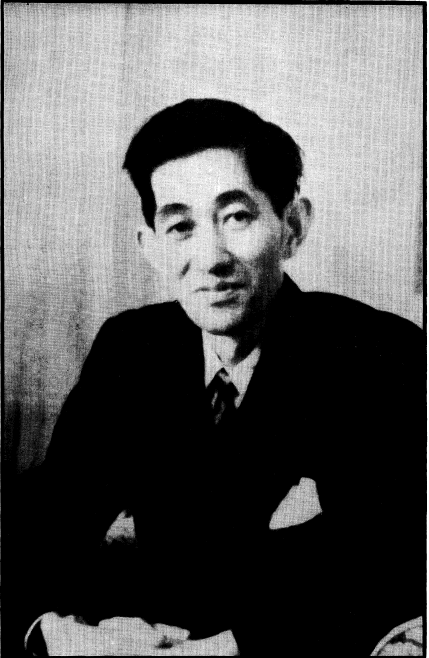
\includegraphics[height=180pt]{Nakayama.png} \\ \vspace{1em}
	\begin{minipage}{0.7\textwidth}
		\small Nakayama's Lemma is named after Tadashi Nakayama (1912---1964). Picture borrowed from \cite{obi-NAK}.
	\end{minipage}
\end{figure}

\begin{corollary}\label{prop:NAK-generation}
	Let $M$ be a finitely generated $R$-module, and let $I \subset \mathrm{rad}(R)$ be an ideal of $R$. If the images of $x_1, \ldots, x_n \in M$ in $M/IM$ form a set of generators, then $x_1, \ldots, x_n$ generate $M$.
\end{corollary}
\begin{proof}
	Apply Theorem \ref{prop:NAK} to $N := M/(Rx_1 + \cdots + Rx_n)$; our assumption $M = IM + Rx_1 + \cdots + Rx_n$ entails that $IN=N$, thus $N=0$.
\end{proof}

We record another amusing consequence of Theorem \ref{prop:NAK}.
\begin{proposition}
	Let $M$ be a finitely generated $R$-module and $\psi \in \End_R(M)$. If $\psi$ is surjective then $\psi$ is an automorphism.
\end{proposition}
\begin{proof}
	Introduce a variable $Y$. Make $M$ into an $R[Y]$-module by letting $Y$ act as $\psi$. Put $I := (Y)$ so that $IM=M$. Theorem \ref{prop:NAK} yields some $Q(Y) \in R[Y]$ satisfying $(1 - Q(Y)Y) M = 0$, that is, $Q(\psi)\psi = \identity_M$.
\end{proof}

\section{Noetherian and Artinian rings}
An $R$-module $M$ is called \emph{Noetherian} (resp. \emph{Artinian}) if every ascending (resp. descending) chain of submodules eventually stabilizes. Recall that in a short exact sequence $0 \to M' \to M \to M'' \to 0$, we have $M$ is Noetherian (resp. Artinian) if and only if $M'$ and $M''$ are. Being both Noetherian and Artinian is equivalent to being a module of \emph{finite length}\index{length}, that is, a module admitting composition series. \index{Artinian}\index{Noetherian}

If we take $M := R$ on which $R$ acts by multiplication, then the submodules are precisely the ideals of $R$. We say that $R$ is a Noetherian (resp. Artinian) ring if $R$ as an $R$-module is Noetherian (resp. Artinian); this translates into the corresponding chain conditions on the ideals. Both chain conditions are preserved under passing to quotients and localizations. Finitely generated modules over a Noetherian ring are Noetherian. The following result ought to be known to the readers.
\begin{theorem}[Hilbert's Basis Theorem] \index{Hilbert's basis theorem}
	If $R$ is Noetherian, then so is the polynomial algebra $R[X_1, \ldots, X_n]$ for any $n \in \Z_{\geq 1}$.
\end{theorem}
Joint with the foregoing remarks, we infer that finitely generated algebras over Noetherian rings are still Noetherian.

On the other hand, being Artinian is a rather stringent condition on rings.
\begin{theorem}\label{prop:Artinian-length}
	A ring $R$ is Artinian if and only if $R$ is of finite length as an $R$-module. Such rings are semi-local.
\end{theorem}
\begin{proof}
	As noticed before, having finite length implies that $R$ is Noetherian as well as Artinian. Assume conversely that $R$ is an Artinian ring. First we claim that $\MaxSpec(R)$ is finite, i.e. $R$ is semi-local. If there were an infinite sequence of distinct maximal ideals $\mathfrak{m}_1, \mathfrak{m}_2, \ldots$, we would have an infinite chain
	\[ \mathfrak{m}_1 \supset \mathfrak{m}_1 \mathfrak{m}_2 \supset \mathfrak{m}_1 \mathfrak{m}_2 \mathfrak{m}_3 \supset \cdots. \]
	This chain is strictly descending, since $\mathfrak{m}_1 \cdots \mathfrak{m}_i = \mathfrak{m}_1 \cdots \mathfrak{m}_{i+1}$ would imply $\mathfrak{m}_{i+1} \supset \mathfrak{m}_1 \cdots \mathfrak{m}_i$, hence $\mathfrak{m}_{i+1} \supset \mathfrak{m}_j$ for some $1 \leq j \leq i$ because maximal ideals are prime. From the Artinian property we conclude that there are only finitely many maximal ideals $\mathfrak{m}_1, \ldots, \mathfrak{m}_n$ of $R$.
	
	Set $\mathfrak{a} := \mathfrak{m}_1 \cdots \mathfrak{m}_n$. Since $R$ is Artinian we must have $\mathfrak{a}^k = \mathfrak{a}^{k+1}$ for some $k > 0$. We claim that $\mathfrak{a}^k = 0$.
	
	Put $\mathfrak{b} := \{r \in R: r\mathfrak{a}^k = 0 \}$, we have to show $\mathfrak{b}=R$. If not, let $\mathfrak{b}'$ be a minimal ideal lying strictly over $\mathfrak{b}$. Thus $\mathfrak{b}' = Rx + \mathfrak{b}$ for any $x \in \mathfrak{b}' \smallsetminus \mathfrak{b}$. We must have $\mathfrak{a}x + \mathfrak{b} \subsetneq \mathfrak{b}'$, for otherwise $M := \mathfrak{b}'/\mathfrak{b}$ is finitely generated (say by $x$) and satisfies $M = \mathfrak{a}M$, then Theorem \ref{prop:NAK} plus $\mathfrak{a} \subset \text{rad}(R)$ would imply $M = \{0\}$, which is absurd. By minimality we have $\mathfrak{b} = \mathfrak{a}x + \mathfrak{b}$. It follows that $\mathfrak{a}x \subset \mathfrak{b}$, i.e. $\mathfrak{a}^{k+1} x = 0$; from $\mathfrak{a}^k = \mathfrak{a}^{k+1}$ we infer $x \in \mathfrak{b}$. Contradiction.
	
	All in all, we obtain a descending chain of ideals
	\begin{align*}
		R & \supset \mathfrak{m}_1 \supset \mathfrak{m}_1 \mathfrak{m}_2 \supset \cdots \supset \mathfrak{m}_1 \cdots \mathfrak{m}_n = \mathfrak{a} \\
		& \supset \mathfrak{a} \mathfrak{m}_1 \supset \mathfrak{a} \mathfrak{m}_1 \mathfrak{m}_2 \supset \cdots \supset \mathfrak{a} \mathfrak{m}_1 \cdots \mathfrak{m}_n = \mathfrak{a}^2 \\
		& \supset \cdots \supset \mathfrak{a}^k = \{0\}.
	\end{align*}
	Each subquotient thereof, which is \textit{a priori} an $R$-module, is actually an $R/\mathfrak{m}_i$-vector space for some $1 \leq i \leq n$. Such a vector space must also satisfy the descending chain condition on vector subspaces, otherwise pulling-back will contradict the Artinian assumption on $R$. Artinian vector spaces must be finite-dimensional. It follows that all these subquotients are of finite length, hence so is $R$ itself.
\end{proof}

\begin{corollary}\label{prop:Artinian-dim-0}
	A ring $R$ is Artinian if and only if it is Noetherian and every prime ideal of $R$ is maximal.
\end{corollary}
\begin{proof}
	If $R$ is Artinian, then $R$ is of finite length, hence is Noetherian as well. For every prime ideal $\mathfrak{p}$, we have $\mathfrak{p} \supset \{0\} = (\mathfrak{m}_1 \cdots \mathfrak{m}_n)^k$ in the notations of the proof above, therefore $\mathfrak{p} \supset \mathfrak{m}_i$ for some $i$, so $\mathfrak{p} = \mathfrak{m}_i$ is maximal.

	Conversely, if $R$ is Noetherian but of infinite length, then the nonempty set of ideals
	\[ \mathcal{S} := \left\{ \text{ideals } I \subsetneq R: R/I \text{ has infinite length} \right\} \]
	contains a maximal element $\mathfrak{p}$. We contend that $\mathfrak{p}$ is prime. If $xy \in \mathfrak{p}$ with $x,y \notin \mathfrak{p}$, then $R/(\mathfrak{p}+Rx)$ has finite length by the choice of $\mathfrak{p}$; on the other hand, $\mathfrak{a} := \{ r \in R: rx \in \mathfrak{p}\} \supsetneq \mathfrak{p}$ (as $y \in \mathfrak{a}$), hence $R/\mathfrak{a}$ has finite length as well. From the short exact sequence $0 \to R/\mathfrak{a} \xrightarrow{x} R/\mathfrak{p} \to R/(\mathfrak{p}+Rx) \to 0$ we see $R/\mathfrak{p}$ has finite length, contradiction.
	
	If we assume moreover that every prime ideal is maximal, then for the $\mathfrak{p}$ chosen above, $R/\mathfrak{p}$ will be a field, thus of finite length. This is impossible.
\end{proof}

Rings whose prime ideals are all maximal are said to have \emph{dimension zero}, in the sense of Krull dimensions; we shall return to this point in \S\ref{sec:Krull-dimension}.

\section{What is commutative algebra?}
In broad terms, \emph{commutative algebra} is the study of commutative rings. Despite its intrinsic beauty, we prefer to motivate from an external point of view. See also \cite{Eis95}.

\begin{asparaenum}[(A)]
	\item \textbf{Algebraic geometry}\index{variety}. To simplify matters, we consider affine algebraic varieties over an algebraically closed field $\Bbbk$. Roughly speaking, such a variety is the zero locus $\mathcal{X} = \{ f_1 = \cdots = f_r = 0 \}$ in $\mathbb{A}^n = \Bbbk^n$ of $f_i \in \Bbbk[X_1, \ldots, X_n]$. The choice of equations is of course non-unique: what matters is the ideal $I(\mathcal{X}) := \{ f \in \Bbbk[X_1, \ldots, X_n] : f|_{\mathcal{X}} = 0 \}$. Conversely, every ideal $\mathfrak{a}$ defines a subset $V(\mathfrak{a}) := \{x \in \Bbbk^n : \forall f \in \mathfrak{a}, \; f(x)=0 \}$. As consequences of Hilbert's Nullstellensatz\index{Nullstellensatz}, which we will discuss later, we have
	\[ V \circ I(\mathcal{X}) = \mathcal{X}, \qquad I \circ V(\mathfrak{a})  = \sqrt{\mathfrak{a}}. \]
	One can deduce from this that the (closed) subvarieties of $\mathbb{A}^n$ are in bijection with ideals $\mathfrak{a}$ satisfying $\sqrt{\mathfrak{a}} = \mathfrak{a}$.

	Furthermore, $\Bbbk[\mathcal{X}] := \Bbbk[X_1, \ldots, X_n]/I(\mathcal{X})$ may be regarded as the ring of ``regular functions'' (i.e. functions definable by means of polynomials) on $\mathcal{X}$, and $\MaxSpec(\Bbbk[\mathcal{X}])$ is in bijection with the points of $\mathcal{X}$: to $x = (x_1, \ldots, x_n) \in \mathcal{X}$ we attach
	\[ \mathfrak{m}_x = (X_1 - x_1, \ldots, X_n - x_n) \supset I(\mathcal{X}). \]
	By passing to the ring $\Bbbk[\mathcal{X}]$, we somehow obtain a description of $\mathcal{X}$ that is independent of embeddings into affine spaces. Moreover, $\mathcal{X}$ inherits the Zariski topology from that on $\Spec(\Bbbk[\mathcal{X}])$.

	Naively speaking, the geometric properties of $\mathcal{X}$ transcribe in ring-theoretic terms to the reduced Noetherian $\Bbbk$-algebra $\Bbbk[\mathcal{X}]$. For example, assume that $f \in \Bbbk[\mathcal{X}]$ is not nilpotent, then the formation of $\Bbbk[\mathcal{X}][f^{-1}]$ corresponds to taking the Zariski-open subset $\mathcal{X}_f = \{x \in \mathcal{X}: f(x) \neq 0 \}$ of $\mathcal{X}$. This may be explained as follows:
	\[ \mathcal{X}_f \simeq \left\{ (x_1, \ldots, x_n, y) : f_1(x_1, \ldots, x_n) = \cdots = f_r(x_1, \ldots, x_n) = 0, \; f(x_1, \ldots, x_n)y = 1 \right\} \]
	which is also an affine algebraic variety in $\Bbbk^{n+1}$, and one may verify that $\Bbbk[\mathcal{X}_f] = \Bbbk[\mathcal{X}][f^{-1}]$.

	\item \textbf{Invariant theory}\index{invariant theory}. Let $G$ be a group acting on a finite-dimensional $\Bbbk$-vector space $V$ from the right, and let $\Bbbk[V]$ be the $\Bbbk$-algebra of polynomials on $V$. Thus $\Bbbk[V]$ carries a left $G$-action by $gf(v) = f(vg)$. For ``reasonable'' groups $G$, say finite or $\Bbbk$-algebraic ones, the classical invariant theory seeks to describe the subalgebra $\Bbbk[V]^G$ of invariants\footnote{More generally, we are also interested in the algebra of invariant differential operators with polynomial coefficients.} in terms of \emph{generators} and \emph{relations}.

	In particular, one has to know when is the algebra $\Bbbk[V]^G$ finitely generated. This is actually the source of many results in commutative algebra, such as the Basis Theorem and Nullstellensatz of Hilbert. For example, let the symmetric group $G = \mathfrak{S}_n$ act on $V = \Bbbk^n$ in the standard manner, then our question is completely answered by the following classical result: $\Bbbk[V]^G$ equals the polynomial algebra $\Bbbk[e_1, \ldots, e_n]$, where $e_i$ stands for the $i$-th elementary symmetric function in $n$ variables.

	The same questions may be posed for any affine algebraic variety $V$. From the geometric point of view, if $\Bbbk[V]^G$ is finitely generated, it will consist of regular functions of some kind of quotient variety $V /\!/ G$. The study of quotients in this sense naturally leads to \emph{geometric invariant theory}, for which we refer to \cite{AG4} for details.
\end{asparaenum}
